%PDF DI RIFERIMENTO: 03_Requirement Engineering.pdf

\chapter{Requirement Analysis}
    \section{Obiettivo}
        In questa sezione verranno analizzate le informazioni definite nei requisiti di sistema al fine di schematizzare opportunamente il dominio del problema.

    \section{Use Case Diagram}
        %Use Case Diagram costruito con StarUML
        \begin{figure}[htbp!]
            \centering
                \vspace{2\baselineskip}
                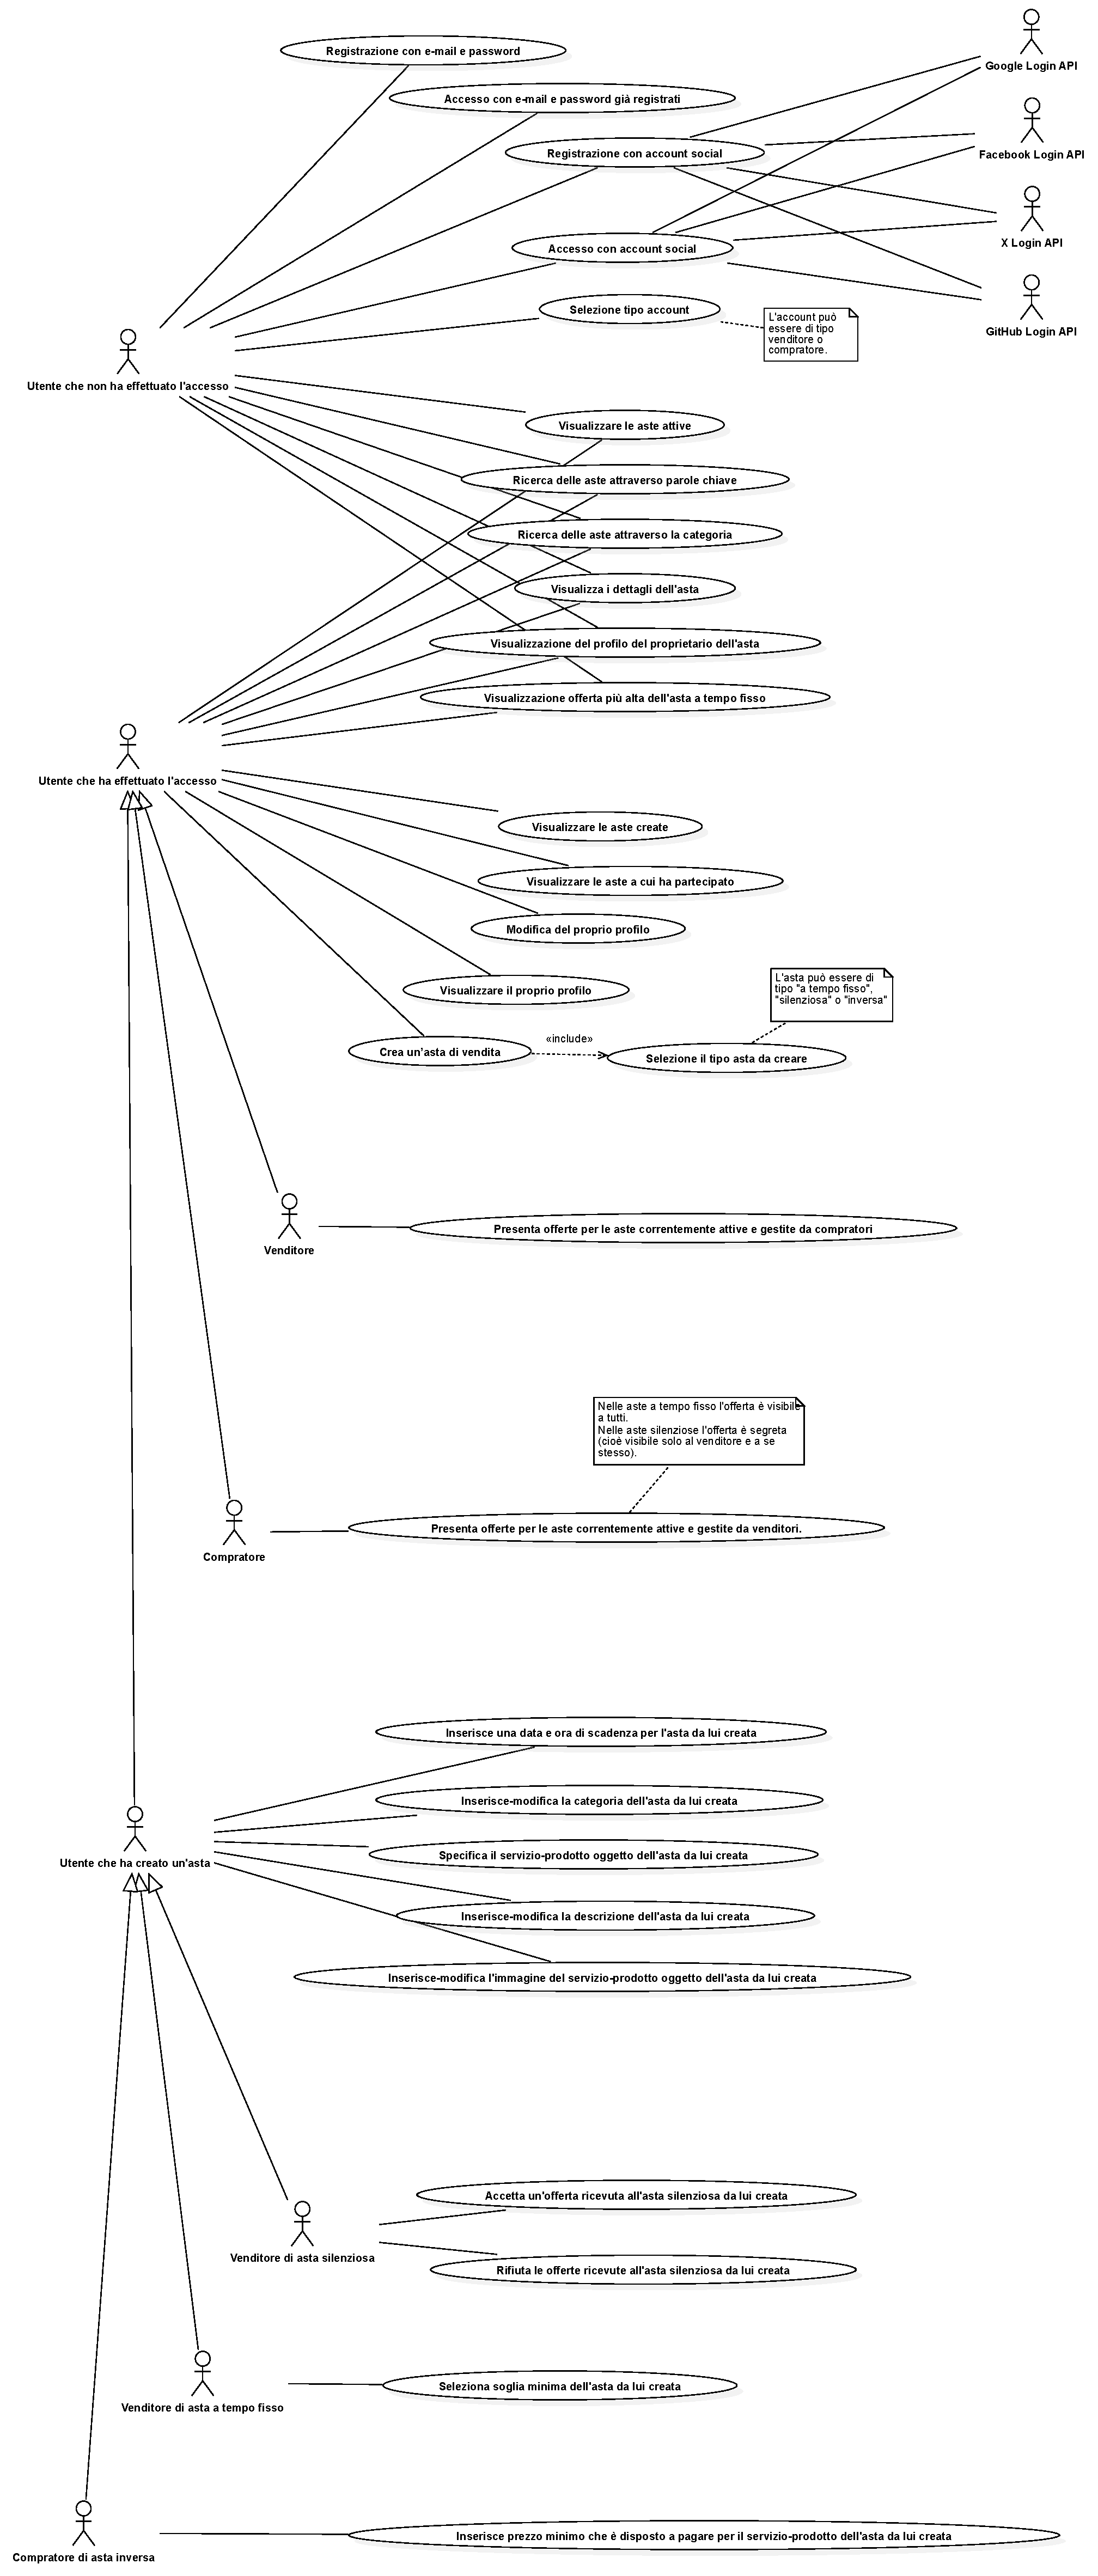
\includegraphics[width=0.35\linewidth]{Immagini/Diagrammi/UseCaseDiagram.pdf}
            \caption{Use Case Diagram}
            \label{fig:Use Case Diagram}
        \end{figure}

    \newpage
    
    \section{Target utenti}
    


    \section{Mockup}

    \section{Tabelle di Cockburn}